%%%%%%%%%%%%%%%%%%%%%%%%%%%%%%%%
\section{Introduction}
\label{sec:compsok:introduction}
%%%%%%%%%%%%%%%%%%%%%%%%%%%%%%%%
% Context: monolithic programs are incompatible with the trust relations within
%         actual components of programs
Modern software architecture, where a majority of applications are monolithic,
stands in stark contrast to the fragmented nature of software development.
Applications run code from diverse authors and varied sources, 
trusted to different degrees, with little to no expression of these trust
relations.
Within a process, all parts of an application execute with the same privileges,
without isolation between parts.
Applications often comprise dependencies and libraries automatically pulled
from software repositories, inheriting the bugs in this software.
Security-critical software can be dynamically extended with third-party modules,
perhaps written by developers lacking the same security consciousness as the
original application's developers.
Further, the code churn over time due to updates of the main application as well
as all of its dependencies makes a comprehensive analysis to eliminate all
bugs or vulnerabilities infeasible~\cite{ZhuB21, LeeSL21}.
Attackers can exploit a bug or malicious code in any component to
compromise the entire application.
Working under the realistic assumption that all code contains exploitable 
vulnerabilities, compartmentalization is a principled approach to 
mitigating the propagation of faults or exploits between components of applications.

% Why compartmentalization works. 
% - assume attacker bypassing other mitigations
% - limit attacker's potential by limiting privileges
Compartmentalization relies on isolating components of applications
within separate compartments,
each with access to the minimal set of privileges to function, preventing
malicious or otherwise unintended interactions between components.
When an attacker compromises any component, exploiting a bug in its code 
and bypassing existing mitigations (for memory safety, for example),
additional restrictions on the compartment's privileges hinders the attacker
by limiting the set of malicious operations they can execute to propagate
and compromise other compartments.
Compartmentalization is based on principles tracing their heritage to 
security research in the 1970s: least privilege~\cite{Saltzer74a} 
and defense in depth.

% Implementing compartmentalization.
% Requires changes in implementation, and defining policy and mechanism.
Compartmentalization fundamentally changes software architecture, requiring
developers to write programs out of well-defined components each of which will
be isolated within a separate compartment with restrictions enforced on each
compartment's privileges.
The definition of compartments and allocation of application functionality to
compartments is specified by a compartmentalization policy.
A compartmentalization mechanism is tasked with upholding the isolation
properties and restrictions defined by the policy.

Identifying the need for compartmentalization, academic and industrial projects
have tried to introduce mechanisms enforcing compartment-wise checks on
operations and resource access.
Proposed mechanisms involve changes to the software~\cite{LittonVE0BD16}, 
hardware~\cite{DuHXZC19XPC,VilanovaBNEV14,SchrammelWSS0MG20Donky,
BhattacharyyaHLGSFP23,ParkLXMK19,ERIMOberwagner19}
or both~\cite{WatsonWNMACDDGL15}.
While these mechanisms are built for compartmentalization, each one targets a
different set of design requirements leading to designs with a significant
range of security and performance characteristics and practicality.
More backward-compatible designs~\cite{ERIMOberwagner19,LittonVE0BD16,ParkLXMK19}
either suffer from high overheads or provide limited security at low
overheads.
With clean-slate designs~\cite{WatsonWNMACDDGL15,BhattacharyyaHLGSFP23,YuWBCS23CAPSTONE}, 
proposals have been able to mitigate these
shortcomings by introducing fundamental changes to hardware/software
interfaces.
However, there is a significant adoption cost for new interfaces,
particularly for hardware, and these proposals are often more exploratory
than practical.
Consequently, there is no accepted standard mechanism to support
compartmentalization, hindering the rate of application adoption.
A comprehensive systematization of compartmentalization mechanisms is
essential to understand the strengths and weaknesses of existing
mechanisms, and to identify the key remaining common shortcomings.

In this paper, we first describe a generic compartmentalized application
and list the attacker model mechanisms attempt to defend 
against (\autoref{sec:compsok:overview}).
Next, we systematically list the avenues for cross-compartment
attacks, and categorize the privileges for operations involved in these
attacks (see \autoref{fig:compsok:attacks}).
We then propose a categorization to classify the restrictions required to 
mitigate these attacks at different points, 
and define security metrics for mechanisms based on how many restrictions 
mechanisms implement and how strong these restrictions
are (\autoref{sec:compsok:properties}).
We also define a categorization for the performance properties of mechanisms
for implementing the checks required to enforce these 
restrictions (\autoref{sec:compsok:practicals}).
Finally, we compare \nmechs mechanisms to find which attacker
models they can protect against, and which restrictions they support
to isolate compartments (\autoref{sec:compsok:evaluation}).
To compare mechanisms quantitatively, we create a scale for
scoring mechanisms' security and practicality, based on their security
properties and their practical limitations including performance overheads.
The scores for each mechanism are illustrated in 
\autoref{fig:compsok:scoring_sec} (security) and 
\autoref{fig:compsok:scoring_perf} (practicality).
We find that
\begin{itemize}
  \item supervisor abstractions (processes and newer proposals) are secure
        but have higher performance overheads,
  \item newer mechanisms are pushing the performance limits of 
        mechanisms, 
  \item clean-slate designs improve the performance-security pareto frontier
        leveraging new interfaces and improved hardware capabilities, and
  \item there are significant areas of missing protections across all
        surveyed mechanisms.
\end{itemize}
Our systematization allows us to gain insights on the range of mechanisms, 
and to highlight improvement opportunities for future mechanisms in 
\autoref{sec:compsok:opportunities}.

%%%%%%%%%%%%%%%%%%%%%%%%%%%%%%%%
\section{Compartmentalization: A Deeper Dive}
\label{sec:compsok:overview}
%%%%%%%%%%%%%%%%%%%%%%%%%%%%%%%%
To understand the security properties of compartmentalization mechanisms,
we need to first understand how compartmentalization expresses trust
relationships within applications, and how privilege restrictions
help enforce isolation as demanded by trust relationships.
Therefore, this section illustrates a practical application as an example
to walk readers through the steps of compartmentalization.

% Why compartmentalize and how
Compartmentalization involves composing applications from communicating 
components with well-defined roles, where each component is restricted to exclusively the 
privileges required to implement their functionality.
To build a compartmentalized program, a developer must identify separate
components in their application, define their privileges, and specify interfaces
allowing communication between compartments respecting the trust relationships
between compartments.
The modern Chromium browser, for example, is compartmentalized into a 
browser kernel and a rendering engine that communicate over 
inter-process communication (IPC) calls~\cite{barth2008security}.
Only the kernel compartment can interact with local system resources like files.
To protect the local system, the kernel compartment distrusts the 
rendering engine compartment which handles sandboxing 
untrusted, and possibly malicious, JavaScript code from websites.
Practically, building a compartmentalized program may rely on a varying mix of
manual programming effort and automated toolchains based on program analysis or
developer annotations.

% Introduce security aspect
The security of compartmentalized programs relies on limiting how compartments
interact, reducing the surface area available for attacks between application
components.
Whereas components of a typical uncompartmentalized, or monolithic, application
can directly interact and affect each other, 
compartments are restricted to only interact via defined and secured interfaces.
Monolithic browsers suffer from severe security issues since code 
compiled from untrusted JavaScript downloaded from a website shares the 
process' address space with key trusted compiler components with
the same access permissions.
Consequently, if a bug in the browser resulted in an arbitrary read/write primitive for
a malicious JavaScript application, that application could directly leak/modify
\emph{any} browser data, or 
execute any code including system calls~\cite{ProvosMMWM07, ProvosMRM08}.
Modern browsers therefore compartmentalize the JavaScript engine and all JavaScript code.
Compartmentalized Chromium removes this interaction by using separate processes,
and hence separate memory address spaces, for the kernel and renderer 
compartments.
An attacker must instead use the more limited IPC interface to exploit separate
bugs in the kernel component to corrupt its memory or execute 
malicious system calls, making similar exploits harder.

% Compartmentalization == restrictions
Compartmentalization mechanisms empower the idea of least privilege by 
enforcing restrictions on which operations each compartment can execute.
Commonly, existing and proposed mechanisms restrict what 
memory compartments may access, what system calls they may use, 
and what supervisor resources compartments may access through those system calls.
For memory access restrictions, mechanisms support either 
separate per-compartment memory address spaces or
per-compartment permissions for intra-address space compartmentalization.
Mechanisms also rely on incarnations of system call filtering to
restrict system calls and access to supervisor resources.
The limitations listed above are not comprehensive: applications may
also require other restrictions such as 
the ability to freeze privileges (essentially limiting temporal permission changes), 
limits on inter-compartment control flow,
the ability for compartments to influence other compartments' register contexts, 
and more.
We will later explore useful restrictions comprehensively in 
\autoref{sec:compsok:properties}.

% Why mechanisms matter
In reality, mechanisms offer varying support for restrictions
and their security properties differ as a consequence.
For example, some mechanisms integrate support for system call filtering 
(e.g., Donky~\cite{SchrammelWSS0MG20Donky}, ERIM~\cite{ERIMOberwagner19}), while
others provide the supervisor the necessary support (\seccells~\cite{BhattacharyyaHLGSFP23}, 
CHERI~\cite{WatsonWNMACDDGL15}),
and some mechanisms are inherently unable to support this restriction (MPK~\cite{ParkLXMK19}, 
CAPSTONE~\cite{YuWBCS23CAPSTONE}).
The differences arise from different design goals, like prioritizing backward 
compatibility with minimal hardware/software changes over clean-slate designs,
and trading-off security checks for greater performance.

%-------------------------------
\subsection{Example: \browser Compartmentalization}
%-------------------------------
\begin{figure}
  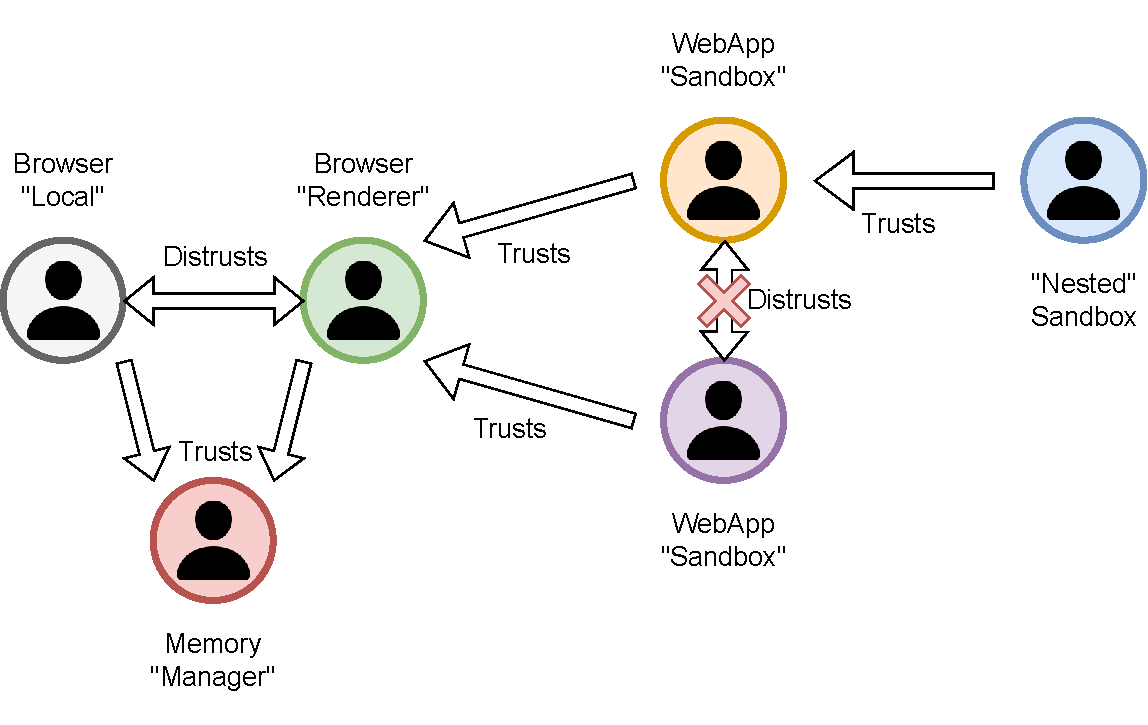
\includegraphics[width=\linewidth]{media/compsok/hierarchy_trust.pdf}
  \caption[Architecture of a compartmentalized \browser]
          {Architecture of a compartmentalized \browser.}
  \label{fig:compsok:browser}
\end{figure}

We shall use a fictional architecture for a browser 
(\autoref{fig:compsok:browser})
to illustrate how the properties of compartmentalization mechanisms 
affect realistic applications.
Our browser roughly resembles a modern Chromium~\cite{barth2008security} 
or Firefox~\cite{wxexclusionfirefox, fffission} browser, 
with separate compartments facing the internet and the local system,
and also includes novel aspects designed to illustrate desirable features
for future applications.

Our \browser is built from compartments implementing different
functionality and executing with the requisite privileges.
The \local compartment is responsible for handling interactions 
with the local system, like accessing files and creating threads.
The \renderer compartment handles the management of sandboxes for running
untrusted code (like JavaScript apps) from websites, including possible
communication between mutually distrustful sandboxes.
The browser isolates web application code from 
separate sources (e.g., separate websites) 
into per-\sandbox compartments.
Finally, we allow a \sandbox to further sandbox a part of itself, effectively
creating a \nested sandbox.
This models the situation where web application developers themselves 
rely on untrusted code, for example, JavaScript code imported by a 
package manager.
A trusted memory \manager compartment handles memory management for the
application and can directly update the system/hardware configuration to 
reflect (de)allocations or permission changes.
The \manager helps model applications with trusted and privileged user 
components directly managing system-level configurations traditionally 
restricted to the supervisor.
Future supervisors, with different compartments responsible for different 
subsystems and having the privilege to modify the relevant system configurations,
may also require support for \manager-like compartments.

\paragraph{Functionality}
Our browser maintains functionality similar to modern browsers.
The \local compartment handles I/O including user inputs and the networking stack, 
and passes inputs for a website over to the \renderer.
The \renderer renders the site, including running the site's dynamic code.
The \renderer either interprets the site's code or creates sandboxes
for running compiled/generated versions of the same code.
Each \sandbox generates website elements while running, which are communicated
to the \renderer. 
The \renderer generates bitmaps visualizing each website and communicates
these bitmaps to the \local compartment which finally sends the image to
the display device.
The \manager handles memory management, ensuring separate regions for 
each compartment when required, and can use privileged operations to
modify hardware configuration as required.
During this process, compartments within the browser communicate by 
calling other compartments and sharing data as arguments.

\paragraph{Threats}
A browser runs code controlled by many parties and manages different threats.
The attacker might control a malicious website and send code when the 
victim uses the browser to access the website crafted to exploit bugs in the
\renderer's code generation engine.
The \browser attempts to protect the local system from such malicious code by
having \renderer and \local components. 
In another attack scenario, a web application generates code attempting to access
a different website \sandbox's data.
Our browser uses per-website Sandboxes to address this threat.
A third attack scenario considers the maintainer of a popular JavaScript package
used by many websites.
The rogue maintainer can make a malicious update to the package which gets
pulled by many unsuspecting website developers, and spread to visitors of many
websites.
The malicious package runs code which tries to access data from the website's
application (perhaps the website user's data) and leaks it as a request to 
another server.
Web developers attempt to mitigate this threat by using \nested sandboxes
for code from untrusted packages.

\paragraph{Trust Relations} 
The browser described above requires various trust relationships.
The \local compartment distrusts the \renderer since it faces the
internet.
For simplicity, we assume that the distrust is mutual, and the \renderer
likewise distrusts the \local compartment.
In this non-hierarchical setup, two compartments must interact without
trusting the other.
The sandboxes, however, create a hierarchy of unidirectional trust where 
the \renderer is trusted by each \sandbox, which in turn are trusted
by their \nested sandboxes.
The \renderer distrusts each \sandbox.
Likewise, each \sandbox distrusts \nested compartments.
The \manager is trusted but distrusts its callers: the \renderer
and \local compartments.

\paragraph{Privileges Expressing Trust Relationships and Functionality}
The browser's compartmentalization policy defines privileges for each
compartment to express the trust relations described above.
A mechanism must implement the restrictions defined below to support
the \browser's requirements.
Each \sandbox must execute in a highly restricted environment, 
maintaining access to defined code and data memory regions and the 
privilege to call into the \renderer to request services like
allocating more memory or managing \nested compartments.
Each \sandbox must be allowed to only call the \renderer and its
\nested sandboxes.
The \renderer and \sandbox{}es (including \nested sandboxes) are all prohibited
from using arbitrary system calls.
% The \renderer might be granted the additional privilege to request anonymous
% memory from a memory management compartment.
The \renderer can implement its functionality, like drawing to the screen,
by requesting services from the \local compartment.
However, the \renderer is trusted by each \sandbox, and is allowed to 
directly access their memory regions including modifying their code.
The \local compartment has greater privileges to use generic system calls.
However, the \local compartment must be restricted to also filter out 
system calls which enable direct access to the 
\renderer{}'s resources (like memory).
An untrusted caller must be prevented from controlling the callee's register
context after a cross-compartment call.
Therefore, a secure context switch is required when calling from the \renderer
into the \local compartment, but is unnecessary when the \renderer calls into a
\sandbox.
To prevent side-channel attacks, specific compartments, like the \sandbox{}es,
must be restricted from executing
microarchitecture-management instructions (like x86's \Code{clflush}) or
reading specific (high-precision) timers.
Since the \manager compartment can modify memory configuration, 
only that compartment should be allowed to execute instructions that change 
privileged registers, access permission tables, and/or maintain hardware 
permission cache (e.g., translation-lookaside buffer or TLB) coherence.

\paragraph{Performance}
Our \browser must be able to provide a responsive browsing experience to its 
users, while incurring overheads from the supporting mechanism associated with 
checks implementing the restrictions described above.
Since applications have performance targets, developers seeking to introduce 
security through compartmentalization must architect their programs considering 
the overheads of the underlying mechanism.
The \sandbox{}es and \nested libraries have short execution periods, and
cross-compartment calls can execute in sub-microsecond timescales.
The \manager compartment must manage (de)allocations equally quickly, to
match web application performance.
Consequently, our \browser demands a proportionally fast mechanism.
To run on slower mechanisms, we must redesign our browser with larger 
compartment which execute longer.
The coarse-grained compartmentalization employed by the Chromium browser
is a result of the significant microsecond-scale overheads of 
compartmentalization~\cite{LittonVE0BD16} built on 
traditional processes (besides factors like code complexity).
Chromium must limit switches between its compartments, since each
inter-process call (IPC) typically costs around ten microseconds.

Higher-performance use-cases for compartmentalization also exist, pushing
the need for mechanisms supporting crucial operations like checks on 
memory accesses, compartment switching, memory (de)allocation, and 
permission changes/transfers/revocation within hundreds, tens, or even single
nanoseconds/cycles.
Server applications are prime candidates for improved security from 
compartmentalization, and are are composed of smaller (often micro-) services,
each of which executes under strict microsecond-scale latency/quality-of-service 
targets.
At datacenter scales, even microsecond-scale delays in a few components can 
balloon into perceptible changes for the end user~\cite{LiSPG14, DeanB13}.
The performance characteristics of mechanisms are of paramount importance to
developers considering compartmentalization for datacenter applications.

%-------------------------------
\subsection{Execution Model and Threat Model}
\label{sec:compsok:threatmodel}
%-------------------------------
We assume that the system being protected is a modern general-purpose CPU
or system-on-chip.
Particularly, the system contains one or more general-purpose 
processors (called cores) and specialized processors (called accelerators).
Processors may be time-shared between different applications and
between different compartments of the same application.
Processors have private hardware resources (like caches) and
shared hardware resources (shared caches, network-on-chip, main memory).
The use of or access to special 
resources (like timing units, devices, or shared registers) requires
special instructions or system calls to privileged supervisor software.
The trusted computing base (TCB) includes the hardware, the 
supervisor software (unless specified otherwise),
and (occasionally) privileged userspace libraries.

The system executes a compartmentalized application, consisting of
communicating compartments executing as per a secure and well-defined 
compartmentalization policy which defines privileges for each compartment.
The policy must be secure, as insecure policies allow applications to be
compromised irrespective of the underlying mechanism, and would not allow
us to compare mechanisms' properties.
We also assume that the application has been initialized properly, i.e.,
that the software-hardware configurations express the correct
compartments, and correct per-compartment privileges to the extent permitted
by the mechanism. 
We assume that compartments secure their communication interfaces, the 
primary remaining attack surface, with necessary checks to prevent 
confused-deputy attacks.
The above assumptions mean that compartments cannot be compromised using 
any sequence of legitimate calls into the compartments
(indicating a shortcoming in the compartmentalization policy, not the
mechanism).
We assume that the developer tries to reasonably implement the same
checks across mechanisms.
For example, consider two mechanisms which check memory permissions for 
4KB pages and byte-granularity objects, respectively.
A developer can reasonably isolate data from two compartments by assigning them
to separate 4KB pages on the first mechanism.
However, developers will consider the memory overhead of assigning each
object on a separate page unreasonable, preventing access control between
two objects on the same page.

We consider an attacker who controls the code and/or data accessible to a
"compromised" compartment of the target application.
The attacker aims to compromise the other compartments of the application,
to either corrupt their execution (integrity) or leak 
information (confidentiality).
The attacker must exploit a weakness of the compartmentalization mechanism,
not the policy.
The attacker can also try to maliciously influence the victim's execution
environment, including the core's microarchitectural state.
The attacker is allowed to execute any operation permitted by the mechanism,
as per the policy.
Executing ISA instructions, special register accesses, and system calls are 
examples of possible operations.
The attacker might attempt to:
\begin{inparaenum}[\itshape i) \itshape]
  \item execute specific instructions including special instructions like
        system calls or permission modification instructions,
  \item access/modify specific resources including virtual memory addresses, 
        physical memory addresses, supervisor resources, and/or physical resources,
  \item execute instructions or operations with specific operands.
\end{inparaenum}

%%%%%%%%%%%%%%%%%%%%%%%%%%%%%%%%
\section{Mechanisms Implement Restrictions}
\label{sec:compsok:properties}
%%%%%%%%%%%%%%%%%%%%%%%%%%%%%%%%
\begin{sidewaysfigure}[]
  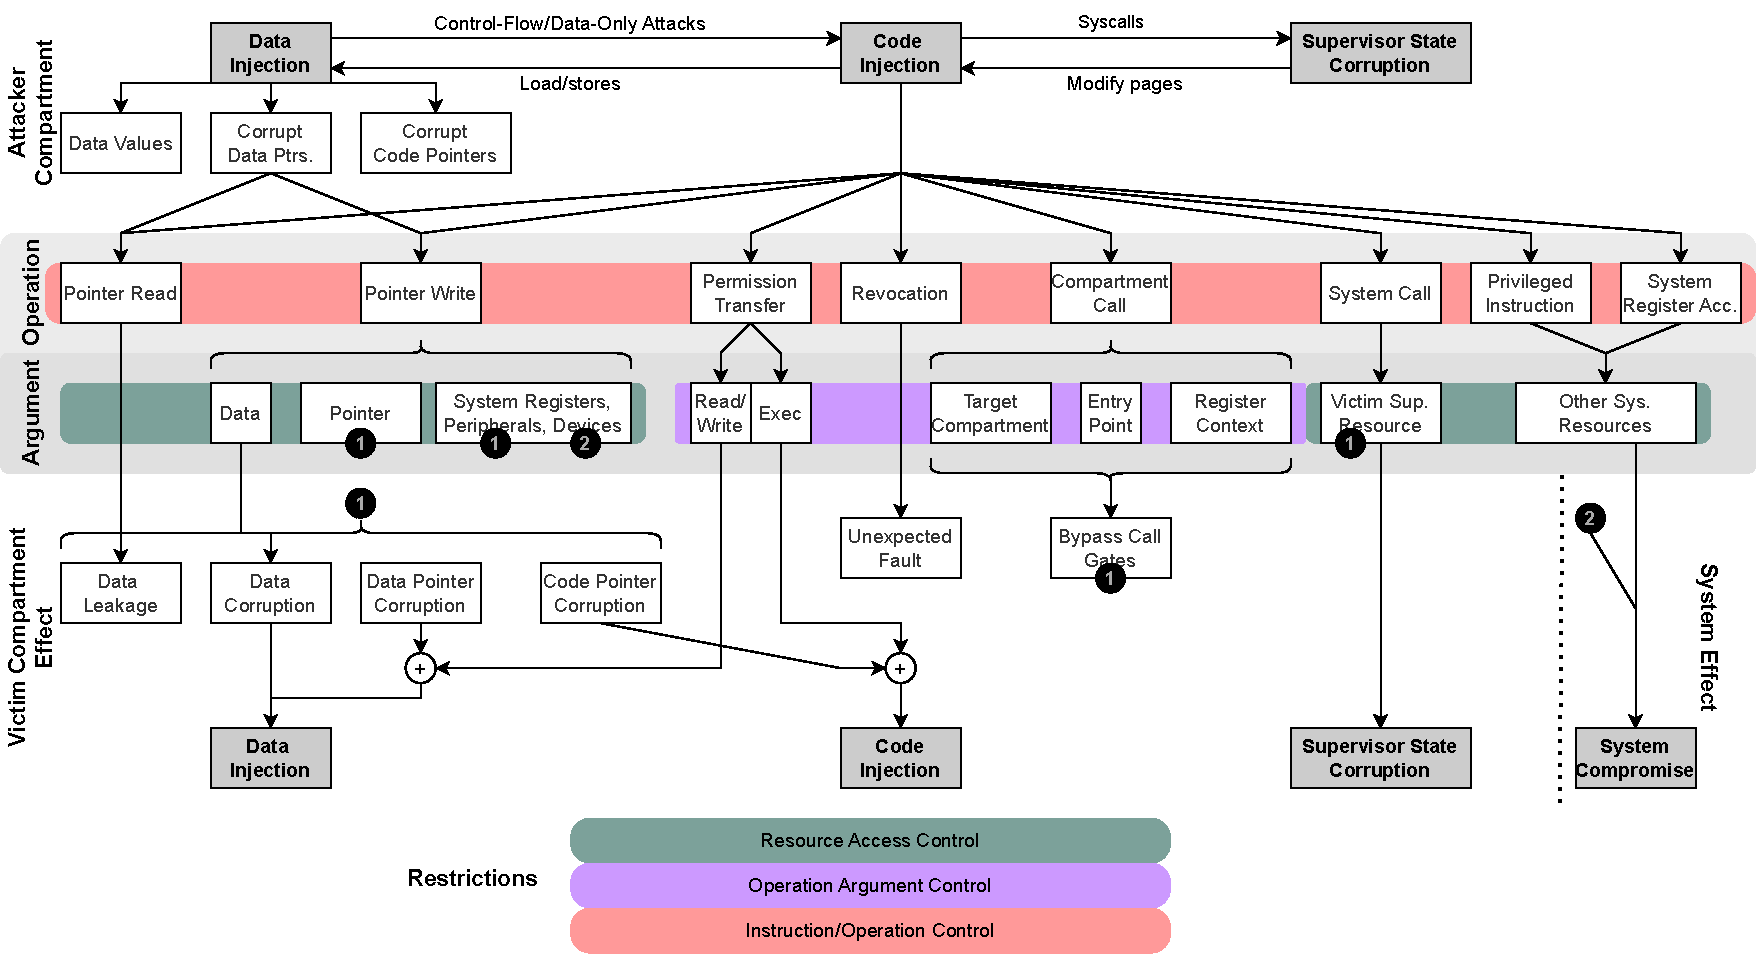
\includegraphics[width=\linewidth]{media/compsok/attacks.pdf}
  \caption[Classification of operations leading to a cross-compartment attack.]
          {Classification of operations leading to a cross-compartment attack, and
          illustration of classes of mitigating restrictions.}
  \label{fig:compsok:attacks}
\end{sidewaysfigure}

Compartmentalization mechanisms support the least privilege principle 
by restricting the abilities of individual compartments.
Attackers rely on an arsenal of different abilities which can allow them
to maliciously leak or corrupt a victim compartment.
In \autoref{fig:compsok:attacks}, we show how an attacker executing
within a compromised compartment can try to compromise other compartments
or the executing system.
In the figure, we highlight the classes of restrictions that mechanisms can 
implement to prevent cross-compartment attacks.
Mechanisms can either limit the instructions or operations that a compartment
can execute, limit the resources accessible by using operations, or
limit the range of arguments that compartments can use for operations.

\begin{table}
  \centering
  \begin{tabular}{l| ll}
    \toprule
    \rowstyle{\bfseries}
    Privilege                   & Type and Restriction Summary                              \\
    \midrule
    \multirow{5}{*}{Resource}   & Virtual memory                                            \\
                                % & Alignment/granularity for VM permissions                  \\
                                % & Number of permission-controlled VM regions                \\
                                % & Exclusive access to VM                                    \\
                                & Physical memory                                           \\
                                & Supervisor resources, e.g., file handles                  \\
                                % & Sup. resources, e.g., files, network devices              \\
                                & System resources, e.g., RNG, timers                       \\
                                & Register contexts                                         \\ \hline
                                % & Timers                                                    \\ 
    \multirow{5}{*}{Arguments}  & Mem. access type (read/write/execute)                     \\
                                & Inter-compartment call target                             \\
                                & Compartment entry point, for call gates                   \\
                                & Perm. transfers: perms., target, granularity              \\
                                & Permission revocation type                                \\ \hline
    \multirow{5}{*}{Operations} & Microarch. configuration (e.g., \Code{clflush})           \\ 
                                & System calls/Traps to the supervisor                      \\
                                & Permission mod./transfers/revocation                      \\
                                & Cross-compartment calls                                   \\
                                & Memory (de)allocation                                     \\ \bottomrule
  \end{tabular}
  \caption{Summary of privileges restricted by compartmentalization mechanisms} 
  \label{tab:compsok:abilities}
\end{table}

% \begin{figure}
%   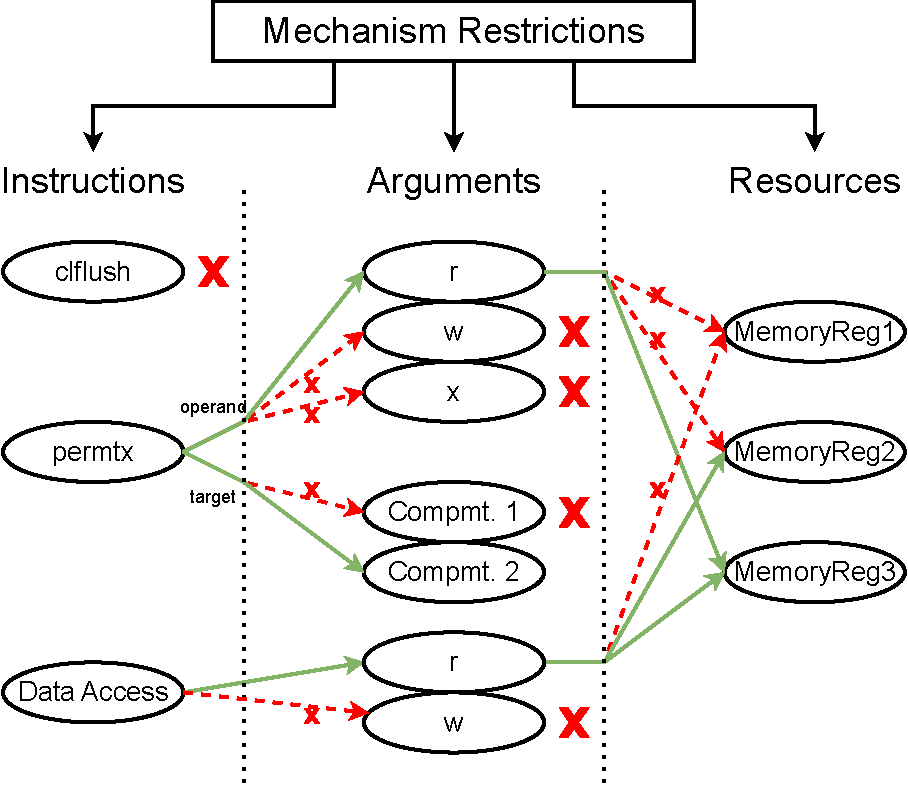
\includegraphics[width=\linewidth]{media/compsok/restrictions.pdf}
%   \caption[Illustrating Restrictions from Compartmentalization]
%           {An example of restrictions implementable by mechanisms. 
%             Resource access control limits read instructions to the latter two memory
%             regions.
%             Operand control limits the \Code{permtx} operation to only transfer 
%             read permissions to Compartment 2.
%             Instruction control restricts the \Code{clflush} instruction altogether.
%           }
%   \label{fig:compsok:restrictions}
% \end{figure}

In this section, we describe abilities available for compartments, whose
use might be limited by compartmentalization mechanisms.
These abilities are summarized in \autoref{tab:compsok:abilities}.
Generally, abilities are classified into restrictions on
\begin{inparaenum}[\itshape i )\itshape] 
      \item resources accessible through instructions or operations,
      \item arguments to instructions, and
      \item instructions/operations compartments can execute.
\end{inparaenum}
We discuss each of these abilities below.
% , and illustrate an example of restrictions
% in \autoref{fig:compsok:restrictions}.

%-------------------------------
\subsection{Resource Access}
%-------------------------------
Applications require restrictions to limit resources accessible to 
compartments, aimed at preventing cross-compartment corruption where
one compartment can directly access to leak or modify other compartments'
resources.
For example, each \sandbox in our \browser is only allowed access to its own 
private state, holding the
values of the objects being used by the website code running in that \sandbox.
An attacker in a different compromised \sandbox with an arbitrary 
read/write primitive can attempt to access a target \sandbox's data directly.
One website running code from an attacker-controlled website 
might attempt to read the login password used for a different website running
in a separate tab temporarily stored in memory, for example.
Alternatively, the attacker might try to access files on the host system's
disk, either to read private files used by other compartments or to compromise
the host system itself.
The mechanism should prevent both of the above attacks.
In \autoref{fig:compsok:attacks}, we show how attackers can attempt to 
dereference corrupted pointers to read/write across compartments and
use system calls to access prohibited supervisor resources.

Common resources requiring access control include virtual memory (VM), 
supervisor resources, access to input/output interfaces, and special registers.
Sandboxes, for example, must be limited to only have access to their own
data and code regions.
Therefore, virtual memory permissions are a key aspect of 
intra-address space compartmentalization mechanisms.
The alignment and granularity requirements for virtual memory permissions
greatly determine a mechanism's security.
Kernel resources, including files, networking, or devices, are also crucial
for isolating compartments.
Essentially, the two aforementioned restrictions stem from restrictions on
the resources accessible through load/store instructions and system calls,
respectively.
Mechanisms might also restrict resources accessible through input/output
instructions.
However, the ubiquity of memory-mapped I/O allows mechanisms to also restrict
I/O by restricting memory access.
Alongside virtual memory, mechanisms might also rely on restricting access to
physical memory regions to prevent concurrent access to data due to aliasing
in virtual memory translations.
Since the execution of compartments is often temporally multiplexed on
the same physical thread running on a core, compartments might also ensure
isolation of register contexts available to compartments.
Finally, compartmentalization might restrict access to system-wide or privileged
resources or registers such as random number generators or those controlling 
permissions (e.g., RISC-V's Physical Memory Protection registers).

%-------------------------------
\subsection{Operation Arguments}
%-------------------------------
Applications also require limits on how compartments are allowed to use
available operations.
\autoref{fig:compsok:attacks} shows how operation arguments can
help cross-compartment attackers bypass call gates or inject code
and data.
For example, system call filters can implement checks on which calls 
compartments can execute.
Compartments might have permission to use the \Code{write}
system call in Linux for writing to the terminal window but are only 
allowed to write to the \Code{stdout} file descriptor and 
denied access to other open files.
The \sandbox compartment in our example \browser must communicate with the
\renderer compartment, and hence has the privilege to use the 
compartment switch/cross-compartment call operation.
The mechanism might limit the target compartment, ensuring that only 
transitions to the \renderer are allowed while denying attempts to
directly call into other Sandboxes.
Further, when calling into the \renderer, the execution must enter at
predetermined entry points allowing the \renderer to implement call gates.
The mechanism must prevent cross-compartment switches to arbitrary
code points in the target.
A mechanism might restrict permission modification operations so that the
new permissions are lesser than the original permissions, to prevent
privilege escalation.
For mechanisms supporting the transfer of memory permissions between compartments,
similar limits can be applied to prevent arbitrary permission transfers.
Mechanisms can allow permissions to be transferred unilaterally or require
bilateral consensus between the granting and receiving compartments.
Systems supporting permission revocation may limit when granted permissions
can be revoked, and in which order.
Finally, mechanisms could limit permitted operands for
instructions (e.g., x86's \Code{CPUID}, RISC-V's \Code{csrr/w}) for
accessing system resources (e.g., control-status registers in RISC-V)
as per an allowlist.

%-------------------------------
\subsection{Instructions and Operations}
%-------------------------------
Mechanisms might altogether restrict access to ISA instructions or other
operations, to limit non-general purpose computation (e.g., arithmetic)
possible by compartments. 
In \autoref{fig:compsok:attacks}, we show how different classes of
instructions enables different cross-compartment attack vectors.
These restrictions can prevent select compartments from using 
instructions/operations with dangerous effects on the environment.
For example, a sandboxing engine might rely on a mechanism to restrict
sandboxes from executing system calls altogether.
Mechanisms might restrict instructions which
control microarchitectural configurations, such as a cache-line flush
instruction (\Code{clflush}) or processor halt.
Instructions controlling microarchitectural state are crucial for
some microarchitectural side-channel attacks~\cite{YaromF14, gruss16flush}.
Generic compartmentalization can also benefit from mechanisms restricting
the ability to use instructions/operations for modifying, transferring or
revoking permissions to specific compartments to only those compartments
requiring dynamic permission changes, and to instructions triggering
cross-core interrupts.
Compartments requiring deterministic execution might also be barred from
special randomness-generating instructions like x86's \Code{rdrand}, which
might enable attackers to access special shared resources~\cite{RagabMRBG21}
or reverse-engineer the generator seed~\cite{ArgyrosK12, CohneyGH18}.
While traditional architectural privilege levels already restrict which
instructions are available at different levels, compartmentalization can
bring a similar security benefit between userspace compartments.
When offloading traditionally supervisor functions to userspace, mechanisms
must also enable limiting the use of traditionally privileged 
instructions (like flushing TLB entries) to authorized compartments only.
Our \browser would benefit from such a restriction, ensuring that a 
compromised \sandbox with injected code can never modify memory configurations
like the \manager is permitted to.

%%%%%%%%%%%%%%%%%%%%%%%%%%%%%%%%
\section{Practical Considerations}
\label{sec:compsok:practicals}
%%%%%%%%%%%%%%%%%%%%%%%%%%%%%%%%
Using a mechanism to compartmentalize an application leads to the application
inheriting the mechanism's performance overheads and other practical limitations.
These limitations may arise from the architectural design of the mechanism or
from an implementation's microarchitectural limits. 
Limitations can lead to either situations where an application cannot be
supported by a mechanism, or where the application suffers additional
overheads beyond a limit.
In this section, we will discuss various limitations of mechanisms, and what
overhead applications will incur as a result.

\paragraph{Limitations}
Mechanisms targeting a wide range of applications offers the best path
towards adoption, and must support varying use cases, policies and
performance requirements.
Our \browser, for example, spawns a varying number of \sandbox{}es, and
requires mechanisms which can allow for many compartments and many 
memory regions for these compartments.
Our \browser also requires different models of trust, including mutual
distrust and hierarchical trust between compartments.
Mechanisms built for hierarchical trust only are unsuitable.
Other possible limitations are dependence on a specific architecture,
limiting common software practices like code sharing between compartments,
or preventing integration with other orthogonal security mechanisms.

\paragraph{Memory Access Control}
The most frequent check implemented by compartmentalization mechanisms is
access control to memory, for loads/stores and for fetching instructions.
Our example \browser{}'s memory footprint can scale from megabytes to 
gigabytes and beyond, and mechanisms must limit access control overheads
in the face of scaling data set sizes.
Modern high-performance desktop and server cores are highly sensitive to
delays in accessing memory, and computer architects strive to enable
fast, single-cycle permission checks.
This criterion has only gained importance since the discovery of the 
Meltdown~\cite{lipp18sec} attack, and 
puts permission checking on the critical path of the memory access to prevent
illegal memory accesses from speculatively leaking data through side channels.
All modern protection mechanisms depend heavily on metadata caching in
microarchitectural structures near the core to enable single-cycle checks in
the common case, and the performance of a mechanism is determined by how 
much data can be accessed through cached permissions.
The performance of permission caching depends on the number of permissions
the mechanism needs to track, which is determined by the granularity of
permission enforcement and the count of individual permissions.
Where mechanisms rely on permissions stored in in-memory data structures
(page table entries, for example, store permissions in a radix tree)
permissions are often cached in lookaside buffers near the core.
The size of these buffers and the size of memory represented by each 
permission entry determines the buffer's reach, i.e., the size of memory
for which permissions can be effectively cached.
Permission tables for fixed-size memory regions like pages 
(traditional virtual memory), hugepages or words require more permission entries 
and incur more costs/overheads than permissions for variable memory ranges,
which can scale to cover arbitrarily large regions.
The choice of granularity of permission also affects performance.
Mechanisms with permission to variable-sized memory ranges can target
storing permissions for each object or for each virtual memory area (VMA).
Applications can require a million times more objects (100's of millions)
vs a few hundred to thousand VMAs.
An alternate class of designs uses hardware capabilities to memory, stored
in memory, and used for validating accesses.
These mechanisms must also be able to validate the access against the
presented capability within a single cycle.
However, capability-based mechanisms typically target per-object capability
storage leading to significant storage overheads and pressure on the
small core-private data caches shared between data and cached capabilities.
Fortuitously, capability systems benefit from the better scaling trends of
L1 data caches compared to TLBs, allowing more permissions to be cached
close to the core.
Alternate capability-based designs storing per-page permissions can scale to
efficiently protect even larger regions.

\paragraph{Compartment Switching}
Compartment switching using inter-compartment calls is expected to also be
a frequent operation, and its latency can significantly affect application
performance.
A \sandbox might use the services of a library in a \nested sandbox
at sub-microsecond timescales.
Assuming fine-grained compartmentalization where small snippets of code, 
corresponding to library calls or sandboxes,
are isolated in compartments, efficiently servicing a sub-microsecond 
cross-compartment call requires the mechanism to support fast compartment
switching within tens or up to a hundred nanoseconds.
Conversely, a mechanism requiring tens of microseconds to switch between
compartments will only efficiently support applications where compartments 
execute for longer timescales (perhaps milliseconds).
Inter-process communication system calls require microseconds on modern
commercial operating systems like Linux or seL4, and this cost limits
compartmentalization for applications like browsers, microservices or 
virtualized network functions in the cloud.
The need for faster switching times is a key motivator for proposals for
alternate OS isolation abstractions and even for hardware-accelerated 
switches.

\paragraph{Instruction Execution Control}
Another conceptually frequent check would be to limit which instructions
a compartment can execute.
Currently, few mechanisms implement such functionality for general instruction
classes.
Only restrictions on instructions based on an executing thread's 
privilege level are widespread.
Restricting instructions might require changes to a core's decode stage, which is
responsible for reading and decoding multiple instructions every cycle on
desktop/server processors.
Given the complexity of the decode stage, modifications might introduce delays 
leading to significant performance overheads.
However, systems with specific use cases might reap sufficient benefit from
delegating common privileged tasks to trusted userspace compartments to justify
this cost.
The \manager compartment, for example, would enable secure memory management
while securely manipulating memory-management unit (MMU) configuration registers.

\paragraph{Exclusive Access}
Certain mechanisms offer additional features, like the ability to maintain
exclusive access to memory regions, transfer permissions to memory regions
between compartments and revoke such grants.
Each of these operations also has a performance cost which will impact
how often applications will use them.
Mechanisms with centralized permission tables and permission lookaside
buffers will suffer the cost of not only modifying permissions, but
propagating these changes between cores to maintain coherence with 
their private lookaside buffers.
In contrast, compartments can transfer permissions by passing capabilities
in registers on supported systems. 
These mechanisms can offer significantly faster permission transfer
operations.
In contrast, revoking granted permissions can be simpler on mechanisms with
a centralized permissions table, which only needs to modify one set of 
permissions when compared to capability-based systems which might need to
scan all memory regions for copies of the revoked capability.
Memory scanning significantly hurts application performance due to large and 
unpredictable delays when a scan is triggered.
Limiting the spread of permission storage within CPU registers or limiting
duplication of capabilities also helps revocation performance.

%%%%%%%%%%%%%%%%%%%%%%%%%%%%%%%%
\section{Evaluating Mechanisms}
\label{sec:compsok:evaluation}
%%%%%%%%%%%%%%%%%%%%%%%%%%%%%%%%
In this SoK, we compare the security and performance characteristics of the 
mechanisms listed below in \autoref{sec:compsok:mechanisms}.
The comparison aims to illustrate common strengths and weaknesses between
mechanisms.
Further, we aim to expose the main missing features that we consider 
useful for future proposals for comprehensive compartmentalization.
We score mechanisms on features introduced in 
\autoref{sec:compsok:properties} and 
\autoref{sec:compsok:practicals}.
The basis for our scores is presented in detail in \autoref{app:compsok:data}
and summarized in \autoref{fig:compsok:scoring_sec} and
\autoref{fig:compsok:scoring_perf}.

%-------------------------------
\subsection{Mechanisms Compared}
\label{sec:compsok:mechanisms}
%-------------------------------
\begin{table}
  \centering
  \begin{tabular}{!l| ?l| ?l| ?l| ?l}
    \toprule
    \rowstyle{\bfseries} 
    Mechanism                              & \makecell{HW/\\Sup} & \makecell{Perm.\\Storage} & \makecell{Runtime\\TCB} & \makecell[l]{Perm.\\Grain}  \\ \midrule
    TRAD                                   & NA                  & PT                        & Sup                     & Fixed          \\
    \lwc~\cite{LittonVE0BD16}              & Sup                 & PT                        & Sup                     & Fixed          \\ 
    CODOMs~\cite{VilanovaBNEV14}           & HW                  & PT+Cap                    & HW                      & Fixed          \\
    XPC~\cite{DuHXZC19XPC}                 & HW                  & PT                        & HW                      & Both           \\
    ARMlock~\cite{ZhouWCW14}               & Sup                 & PT+Reg                    & HW-Sup                  & Fixed          \\
    MPK~\cite{ParkLXMK19}                  & NA                  & PT+Reg                    & HW                      & Fixed          \\
    ERIM~\cite{ERIMOberwagner19}           & NA                  & PT+Reg                    & HW                      & Fixed          \\
    Donky~\cite{SchrammelWSS0MG20Donky}    & Both                & PT+Reg                    & HW-User                 & Fixed          \\
    MMP~\cite{WitchelCA02MMP}              & Both                & PT                        & Sup                     & Range          \\
    \seccells~\cite{BhattacharyyaHLGSFP23} & Both                & PT                        & HW                      & Range          \\
    CHERI~\cite{WatsonWNMACDDGL15}         & Both                & Cap                       & HW                      & Range          \\
    CAPSTONE~\cite{YuWBCS23CAPSTONE}       & Both                & Cap                       & HW                      & Range          \\ \bottomrule
  \end{tabular}
  \caption[Summary classifying compartmentalization mechanisms.]
          {Summary classifying surveyed compartmentalization mechanisms characteristics.
            Columns are described in \autoref{sec:compsok:mechanisms}.
          }
  \label{tab:compsok:summarymechs}
\end{table}

In our SoK, we have tried to include a variety of mechanisms across a variety of
design points.
These mechanisms are listed in \autoref{tab:compsok:summarymechs}.
As our baseline, we include process-based compartmentalization on traditional
operating systems, which is commercially used for software compartmentalization.
Labeled ``TRAD'', our baseline includes traditional monolithic operating systems 
like Linux, FreeBSD, and Darwin as well as commercial microkernels like seL4.
In the ``HW/Sup'', we classify what changes are required for each mechanism.
Among research proposals, we include mechanisms which can run on 
commercial-off-the-shelf hardware with no changes (NA), 
mechanisms requiring supervisor code changes (``Sup''),
hardware modifications (``HW'') or both.
We have chosen mechanisms to span the range from designs targeting full 
backward compatibility to designs aiming for minimal changes to clean slate designs.
Surveyed mechanisms rely on a trusted computing base at runtime dependent on
the supervisor (``Sup''), hardware (``HW'') or even privileged userspace
libraries (``User'').
The variation continues with implementations of permission storage, including
mechanisms relying on variations of permissions tables (``PT''), special
permissions registers (``Reg''), capabilities (``Cap''), or a mix of the
above.
Finally, we find mechanisms using permissions for fixed-size memory regions 
(pages, words), variable-sized regions (objects, segments and virtual memory areas),
and even both.

In our comparison, we have omitted other compartmentalization mechanisms
solely based on software-based checks~\cite{WahbeLAG93} 
which are incapable of protecting against strong attacks as defined in 
\autoref{sec:compsok:threatmodel} as they
do not add any protection beyond that provided by traditional processes.
We have also excluded mechanisms based on 
virtualization~\cite{BelayBMTMK12, KoningCBGA17, LiuZCCX15, McCuneLQZDGP10, SharifLCL09}
as they provide similar protections as processes, 
but at a higher cost and protect against potentially rogue supervisors.
We have also omitted other mechanisms based on novel OS abstractions due to a
lack of space~\cite{HsuHEP16, DautenhahnKDCA15, ChenRSL16, BittauMHK08}.
We also exclude mechanisms abusing non-security hardware features for non-systematic
point protections~\cite{HedayatiGJCSSM19Hodor, GuanLLJW15}.
Finally, we exclude mechanisms with very limited protections~\cite{FrassettoJLS18}.

%-------------------------------
\subsection{Methodology and Rationale}
\label{sec:compsok:methodology}
%-------------------------------
We classify mechanisms on the axes described in 
\autoref{sec:compsok:properties}, essentially trying to measure how well 
each mechanism supports per-compartment restrictions to executable operations,
resources accessible by those operations, and arguments to those operations.
Each mechanism is individually scored on each axis, and the results are shown
as a radar plot (see \autoref{fig:compsok:scoring_sec} and 
\autoref{fig:compsok:scoring_perf}).
To measure a mechanism's score on an axis, we essentially add scores 
corresponding to various restrictions that could be implemented on that axis.
For each restriction, mechanisms are scored by whether that mechanism supports
that restriction, and how well it supports the restriction compared to the 
other mechanisms.
For example, when scoring a mechanism on resource access restrictions, we
add scores corresponding to limits on memory accesses and supervisor resource
accesses.
When scoring mechanisms on virtual memory controls, we consider whether
mechanisms restrict instruction accesses (execute) as well as 
data fetches (load/stores).
For data access, mechanisms that support finer-grained access control checks, 
such as per-object permissions, score more than mechanisms that enforce 
page-granular access control.

%-------------------------------
\subsection{Comparison}
\label{sec:compsok:comparison}
%-------------------------------
\begin{figure}[ht]
  \centering
  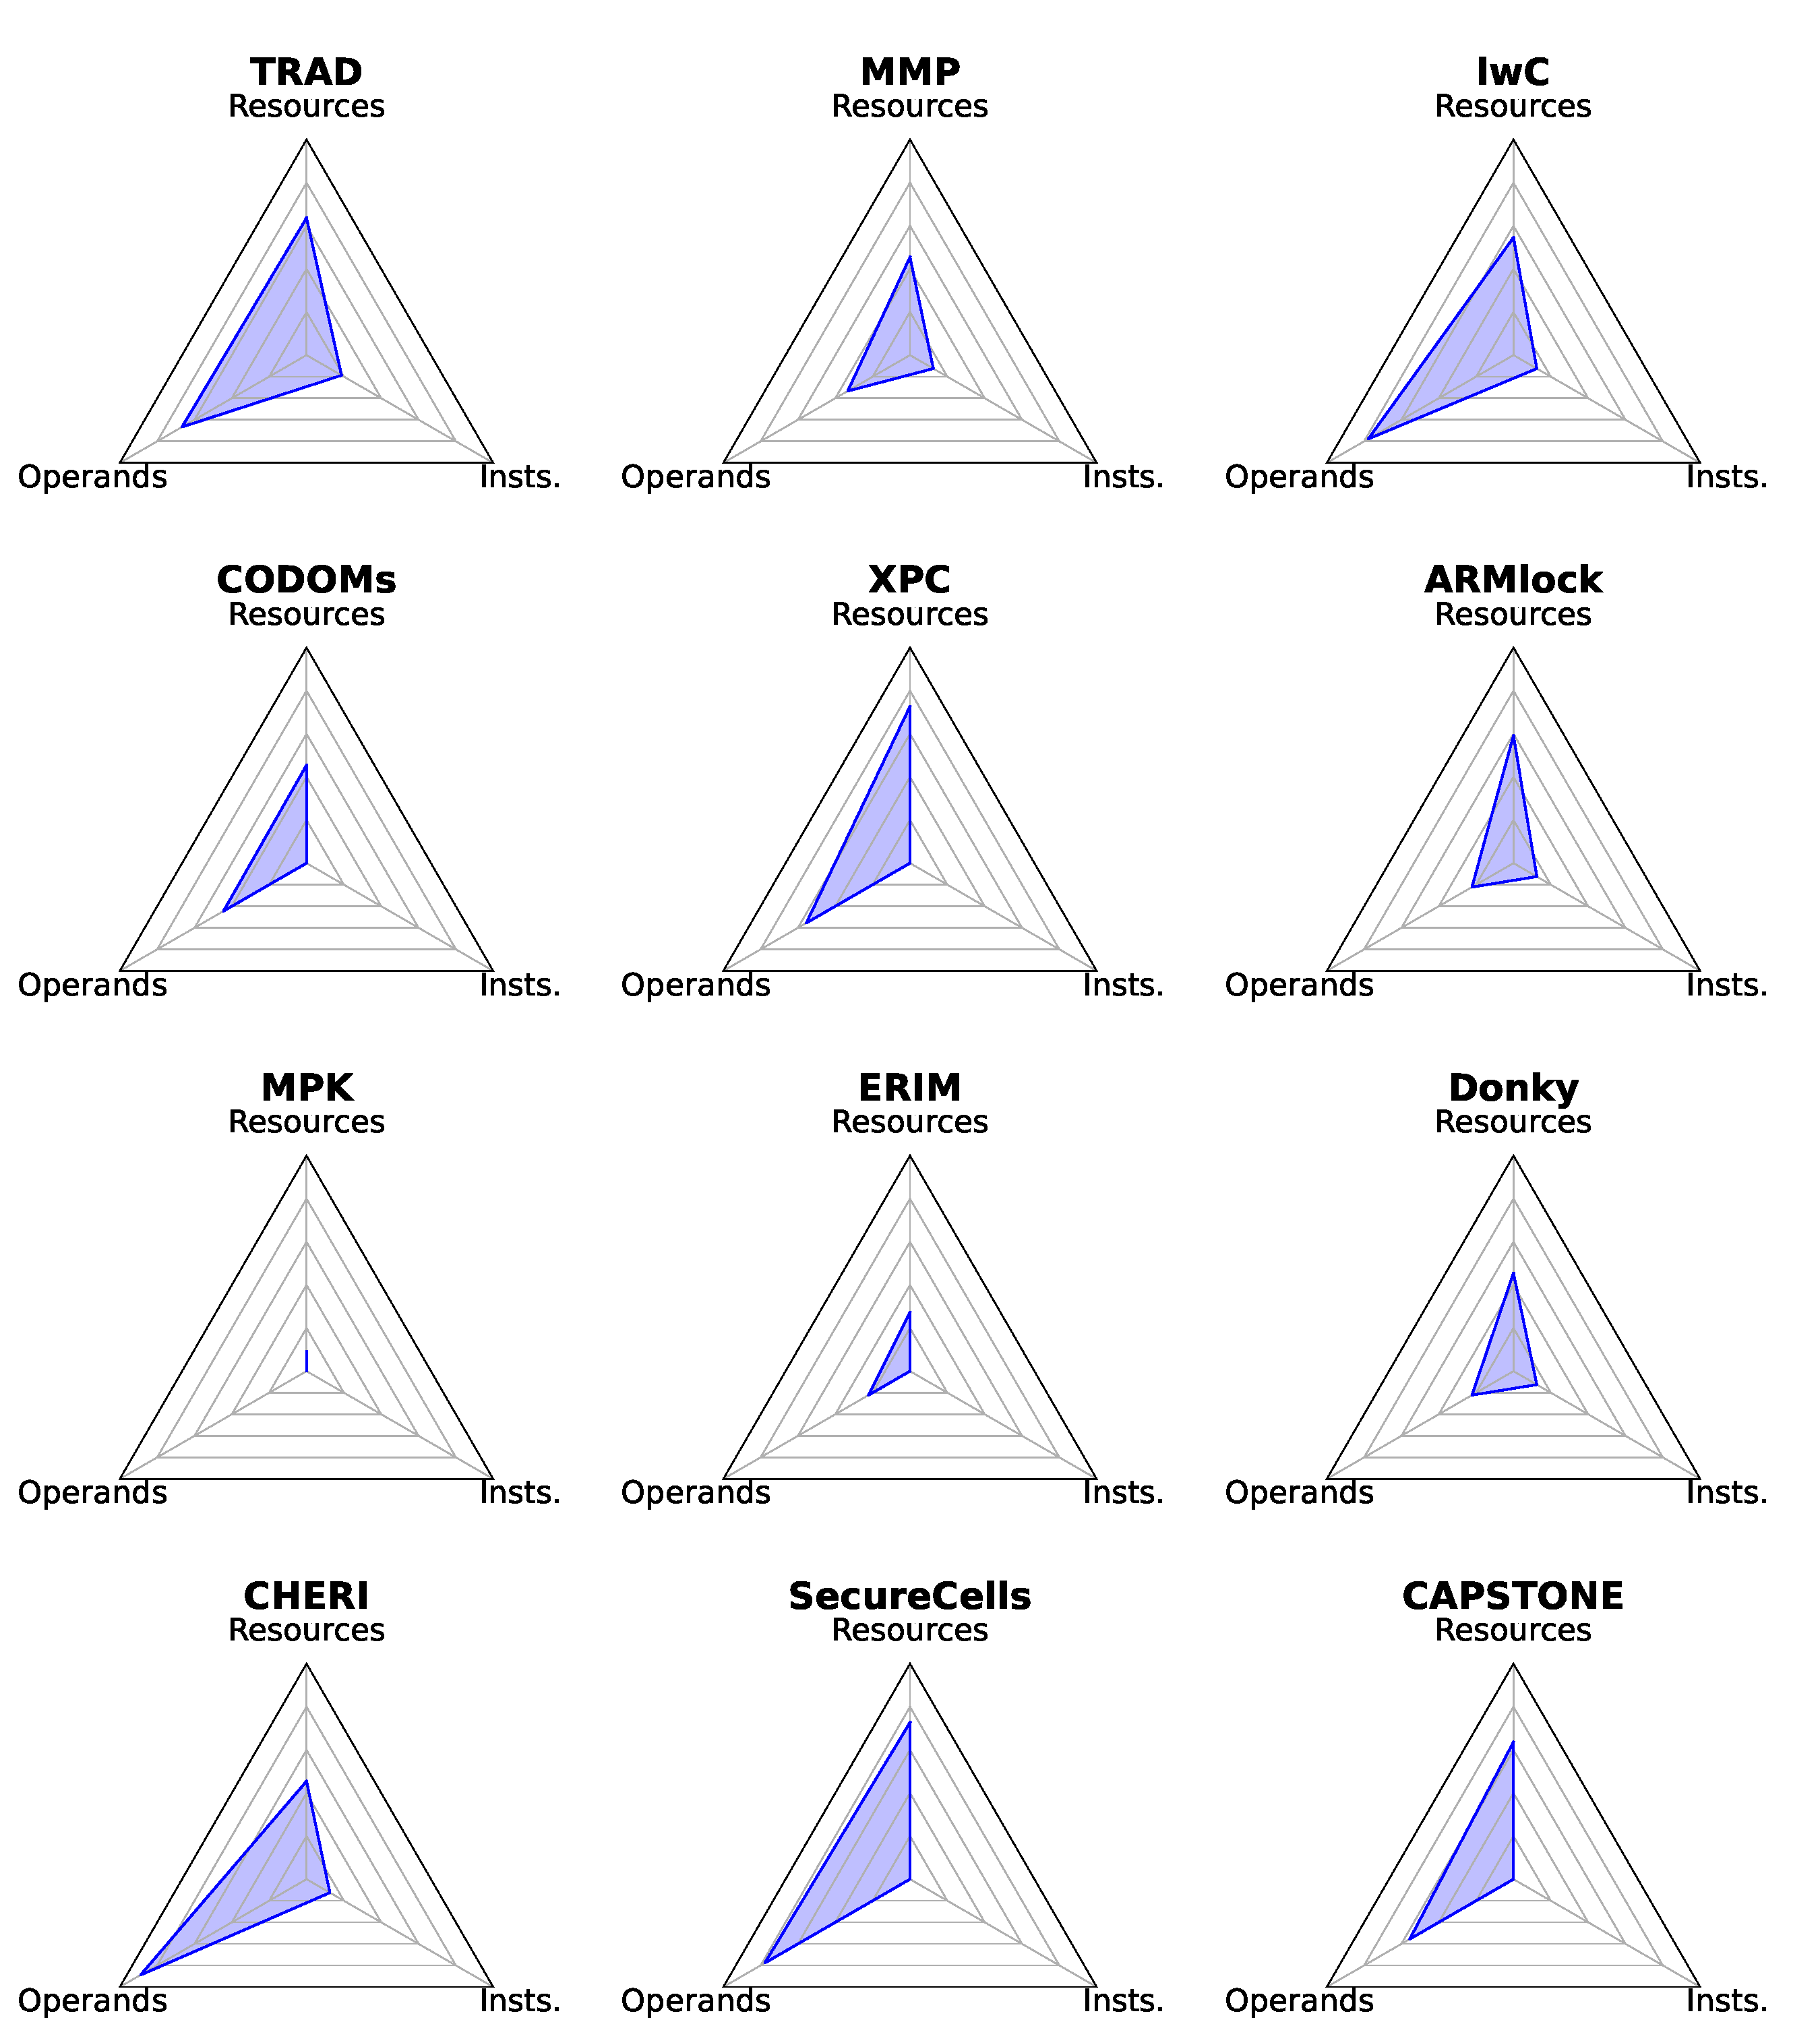
\includegraphics[width=0.9\textwidth]{data/compsok/scoring_security.pdf}
  \caption[Scoring security properties of mechanisms.]
          {Scoring security properties of mechanisms.}
  \label{fig:compsok:scoring_sec}
\end{figure}

\begin{figure}[t]
  \centering
  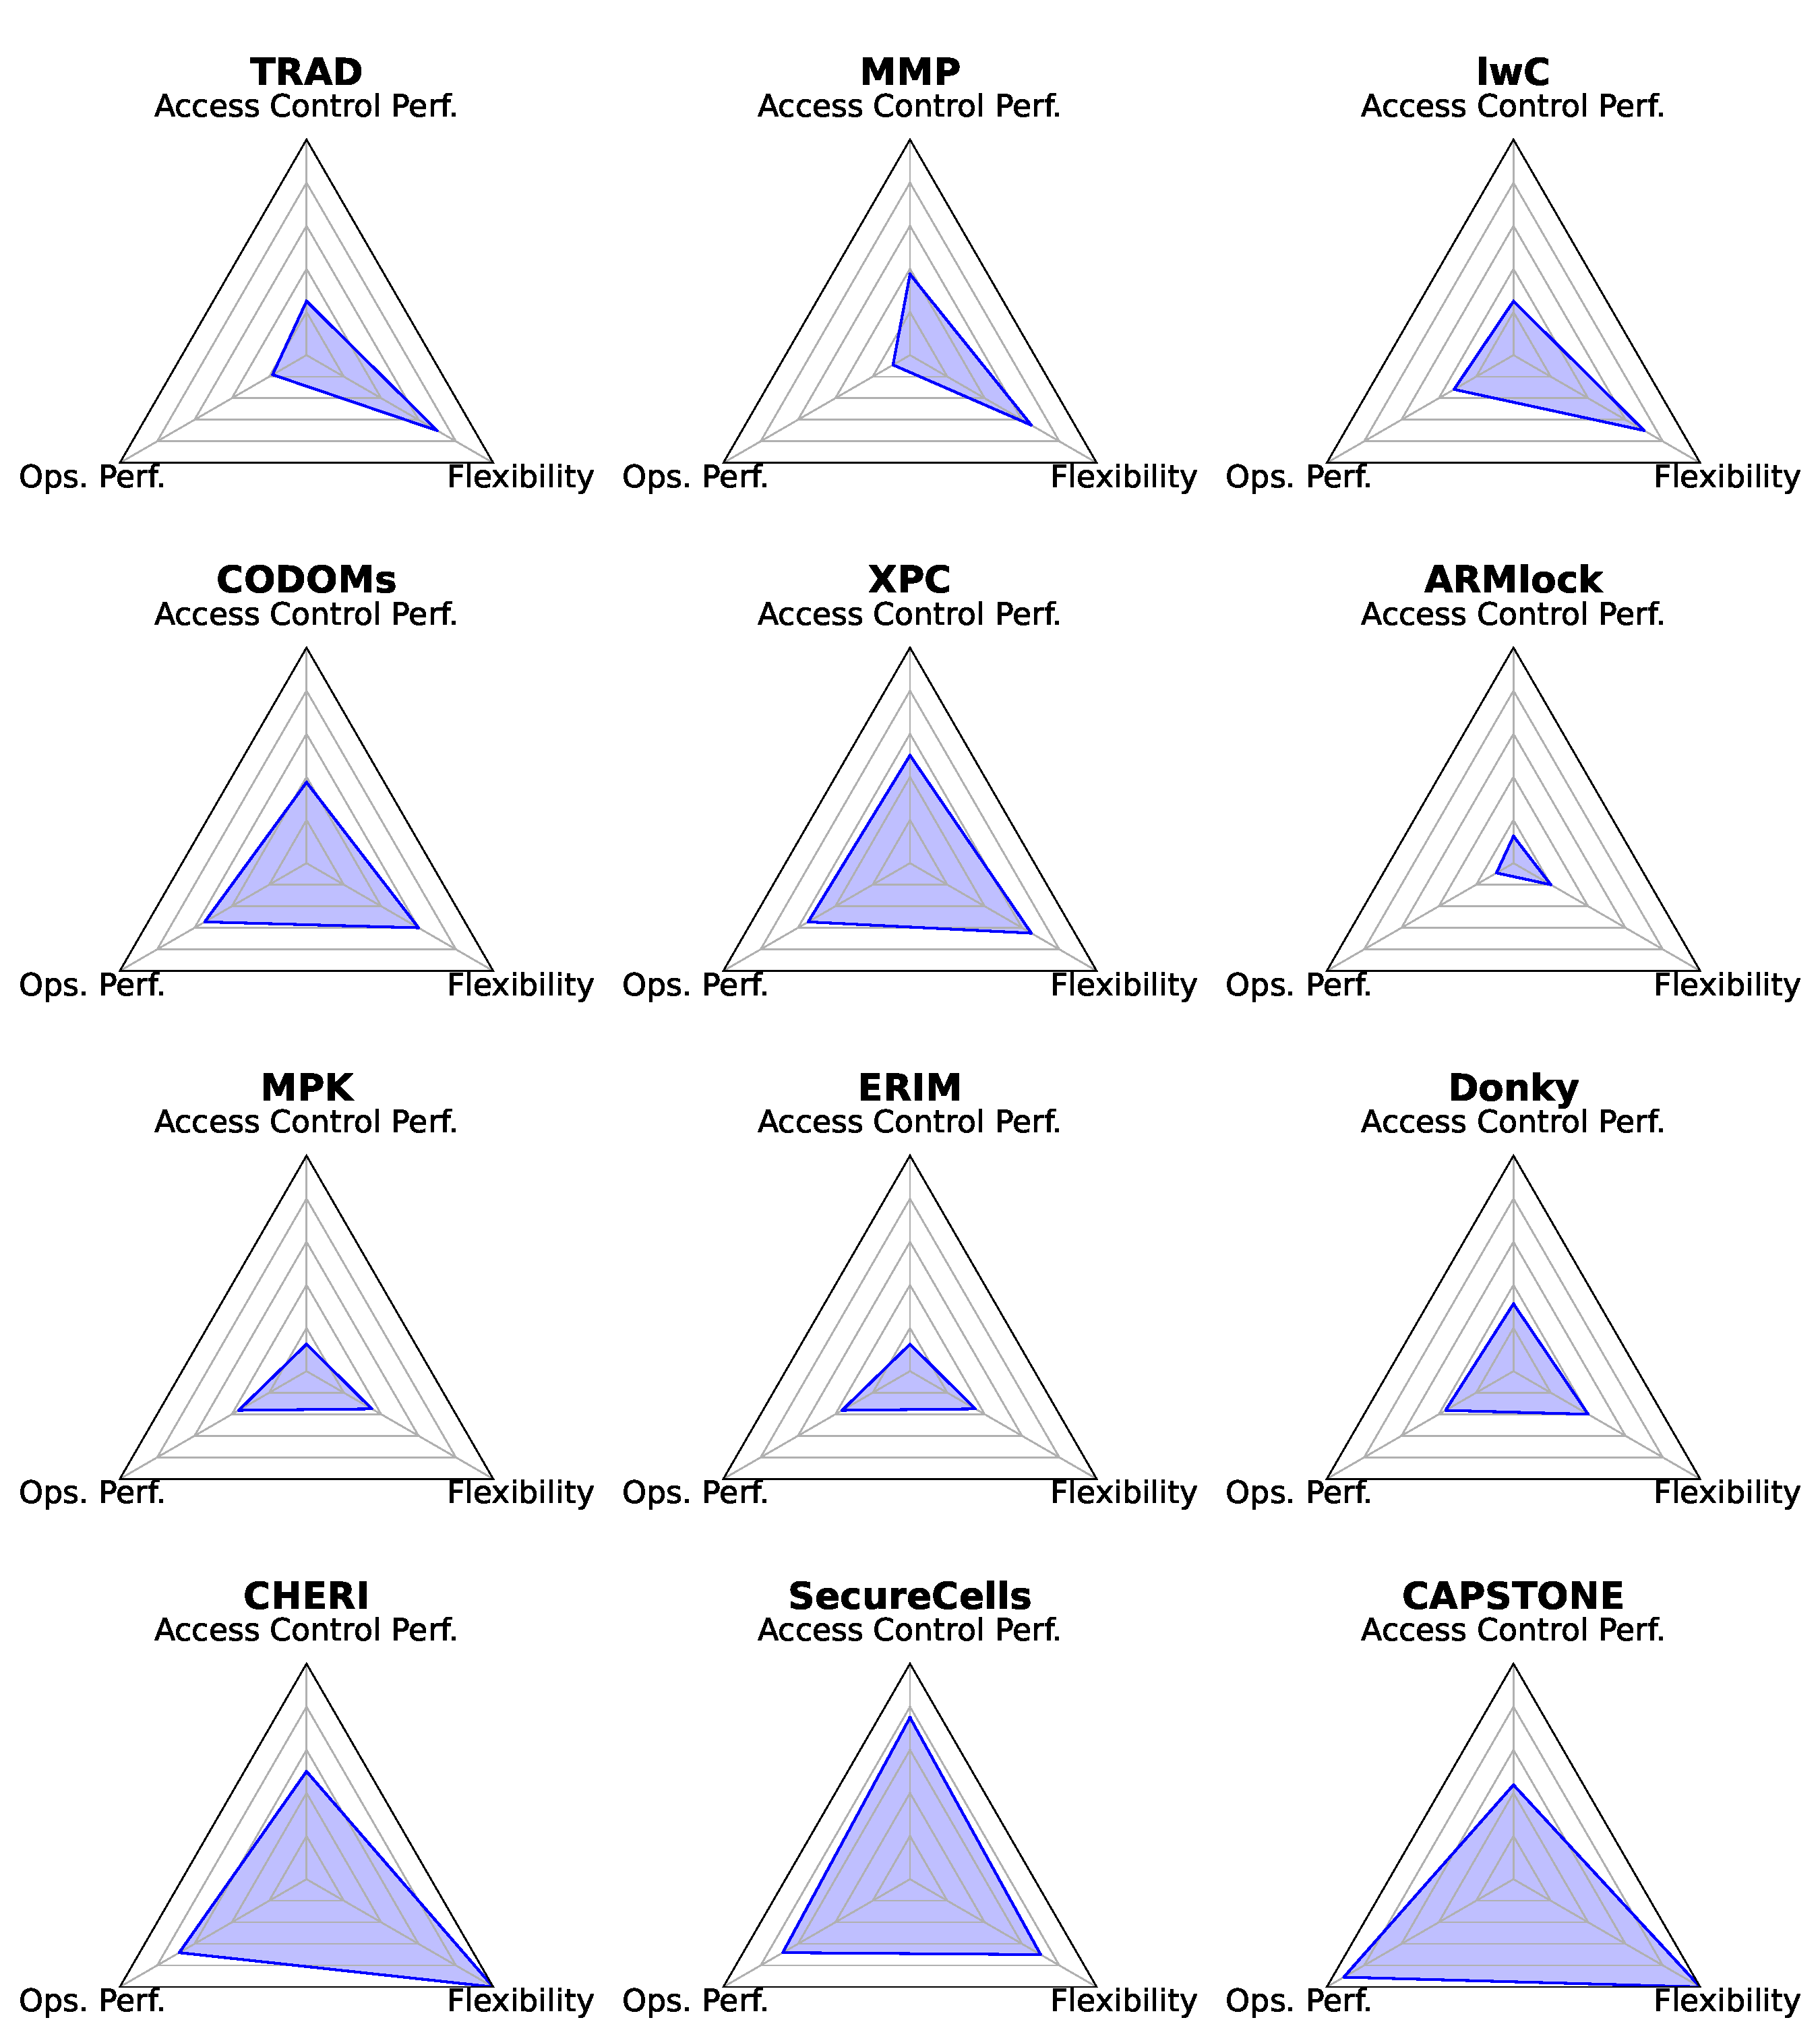
\includegraphics[width=0.9\textwidth]{data/compsok/scoring_practicality.pdf}
  \caption[Scoring practicality and performance aspects of mechanisms.]
          {Scoring practicality and performance aspects of mechanisms.}
  \label{fig:compsok:scoring_perf}
\end{figure}
% \FloatBarrier

The scores for mechanisms on two aspects, security and practicality, 
are illustrated in 
\autoref{fig:compsok:scoring_sec} and \autoref{fig:compsok:scoring_perf},
respectively.
In this section, we focus on insights gained from broadly
comparing mechanisms.
Overall, we find that the most secure mechanisms are designed for strong
attacker models, including using
operating-system abstraction (TRAD, \lwc), capabilities (CHERI, CAPSTONE)
and hardware permission checks (MMP, XPC, \seccells).
Further, hardware changes designed for compartmentalization are essential for
high-performance mechanisms (XPC, CHERI, \seccells and CAPSTONE).

We postulate that a mechanism's design greatly influences its security
characteristics.
Given that mechanisms are designed for different threat models, their
security scores for our powerful attacker model can seem lacking.
Mechanisms targeting strong attacker 
models (TRAD, \lwc, XPC, CHERI, \seccells, CAPSTONE) 
present strong scores on restricting access to resources and operations.
Other mechanisms (CODOMs, MPK, ERIM, and Donky) have simpler designs
trading off security for simplicity and performance.
For example, MPK only checks the data access path. 
A more secure version of MPK, also checking code fetches, would require
changes to the core's (complicated) fetch stage, and require additional
bits in the permissions key register (PKRU) for permission storage.

Access control for memory varies on two factors, the granularity of targeted
permissions and alignment requirements for regions.
Finer, object-level permissions are supported with 
permission tables (MMP, \seccells) but are more suitable for capability systems.
Most permission table-based mechanisms target access control for larger
fixed-size (2MiB, 4KiB or 16KiB) pages or 
memory regions (virtual memory areas in \seccells).
Systems with range-based permissions (MMP, CHERI, \seccells and CAPSTONE) support
memory ranges starting and ending at any byte (or word) boundary.
Meanwhile, page tables also impose a page-sized alignment requirement for
regions of memory.
Fine-grained permissions allow developers to shrink the size of compartments, 
and better isolate components of their applications.
However, the spatial granularity of permissions trades off security and
performance as the mechanism is responsible for tracking and enforcing
permissions for more regions as the granularity of permissions shrinks.
Whereas modern browsers hold hundreds of millions of objects, they use
millions of pages, and thousands of virtual memory areas.
Most mechanisms also support an almost arbitrarily large number of memory
regions.
Key exceptions are mechanisms based on protection keys or page colors.
ARMlock, based on ARM's memory domains feature,
and MPK-based mechanisms support only 16 different colors, and 
Donky improves the limit slightly to support up to
1024 different colors.

Access control to virtual memory is a common feature across most of the
mechanisms considered.
Virtual memory permissions can prevent spatial memory safety violations,
a major and relatively simple attack vector, from propagating
beyond compartments.
Traditional, OS-based mechanisms have a strong score for controls on 
memory access, since compartments are assigned separate processes which present
the abstraction of isolated virtual memory spaces.
Similar high scores are achieved by other research proposals with strong
emphasis on security. 
However, commercial mechanisms trading off performance for security, such as
Intel's MPK and mechanisms built on MPK, show lower scores here.
Particularly, MPK only prevents illegal data access (read/write) to pages
of a different color, protected by a register directly and arbitrarily
writable by userspace.
ARMlock, however, also checks code fetches.
ERIM and Donky improve on MPK's design, adding integrity for compartment
transitions and protection key updates, respectively. 
However, each of these mechanisms scores better than MPK, but still score 
poorly for virtual memory protection due to lacking execute permission
checks and support for exclusive access.
ERIM also lacks of support for context isolation, like MPK.

Support for access control to physical memory is scarce among the surveyed
mechanisms, with only CAPSTONE providing capabilities for physical memory, and
XPC providing a relay segment which the supervisor points to separate per-core
physical memory regions.
Permissions for physical memory alleviate the possibility of attackers leveraging
aliasing in physical-to-virtual address translations to bypass memory protection
and access prohibited physical memory.
Practically, controlling permission to physical memory is inherently difficult
as applications operate with virtual addresses and physical addresses are hidden
from userspace and controlled by operating-system-managed translation tables.
CAPSTONE reveals physical addresses to user applications, possibly simplifying 
attacks on physical memory like Rowhammer~\cite{mutlu2019rowhammer}.
Further, a core designed to perform protection checks on physical addresses 
\emph{after} translation stands to suffer a significant performance hit from
the increased latency to access memory.
RISC-V specifies Physical Memory Protection (PMP) registers, ranges of physical 
memory with specific addresses, but their current design is more suited for
confidential computing than compartmentalization.
PMP registers can only be modified by the machine-mode firmware, and are often
sealed at boot time to predetermined processor-private memory regions.
Instead, future mechanisms can focus on providing guarantees against aliasing
for virtual-physical translations for data regions, preventing this class of
attacks.

Access control to supervisor resources varies more between mechanisms.
Assuming per-compartment system call filtering rules are implemented, the 
supervisor must be able to securely identify the calling compartment to
perform the correct set of checks.
Donky and ARMlock explicitly present system call filtering as part of the 
mechanism.
Mechanisms where compartments switch using a 
system call (TRAD, MMP, \lwc, CODOMs, ARMlock and CHERI) 
indirectly allow the supervisor to identify the caller. 
Linux, for example, stores a pointer to a process' supervisor metadata in a
privileged register when the corresponding user process executes, allowing
the supervisor to identify process on traps.
Mechanisms which explicitly identify the executing compartment (XPC, \seccells)
enable the supervisor to directly identify the compartment.
With Intel's MPK and ERIM, the supervisor may be able to indirectly identify the 
caller by the value of the permission-key register, if unique.
Finally, compartments in CAPSTONE are implicit, relying on capabilities
stored in registers and hardware calls for switching to compartments with
sealed capabilities.
The supervisor has no direct or indirect mechanism to identify the caller, since
the caller's state is also sealed on traps.
CAPSTONE, therefore, cannot implement system call filtering.

We notice that support for restricting per-compartment instructions or
operations are a common shortcoming among most mechanisms.
These restrictions are crucial to enable future systems offloading supervisor
functionality to userspace, primarily for high-performance server
applications, or for compartmentalizing supervisor kernels.
These applications would benefit from limiting system management code with
the corresponding privileges within individual compartments for each
aspect of management (memory, per-device drivers, scheduling).
Only traditional operating systems can selectively disable processor features,
like the x87 floating-point unit, though this feature exists as a side-effect
of power-saving features in the CPU or due to the requirement to disable
faulty CPU functional units.
We notice that researchers focus on memory isolation and build on a simplified
system model with only computing elements (like cores) and memory.
Future proposals should also consider restrictions to the many accessible 
system-wide resources on commercial CPUs.

Mechanisms are also designed to support different classes of applications.
Traditional applications (specially desktop/mobile applications) are 
compartmentalized with processes reusing an existing operating system abstraction
for isolating users and applications running on a shared machine, 
and assume the performance costs of using a mechanism not designed
for fine-grained compartmentalization.
Meanwhile, applications can also benefit from any additional security for
data accesses introduced by commercially available 
mechanisms (MPK, ARM's memory domains).
MPK deliberately enables userspace modification of permissions, as opposed to
the supervisor (ARMlock), for improved performance.
However, high-performance software like supervisor kernels and some server
software require secure but high-performance mechanisms and may be better
supported by research proposals.
Compartments mapped to processes (TRAD, \lwc) use separate address spaces and 
permissions stored in page-table entries to securely isolate memory.
Consequently, page-table entries across compartments share capacity within an 
already size-constrained microarchitectural buffer.
Commercial compartmentalization based on Intel's MPK also use 
page-table entries for storing translations and page colors, 
but rely on permissions stored in the PKRU register, slightly relieving
TLB pressure.
ARMlock slightly alleviates this pressure by storing colors for 2MiB hugepages.
Due to the reliance on TLBs for permission metadata, mechanisms based around
traditional computer architectures and page tables score poorly on performance
for access control to memory.
Two approaches to alleviate this pressure exist.
First, MMP separates permissions from translations, implementing a separate
permissions table and caching buffer.
Second, MMP and \seccells include support for storing permissions to 
variable-sized regions, ideal for separating permissions for virtual memory
areas ubiquitous in modern applications.
Technically, CODOMs removes TLB pressure by only allowing a single compartment
access to each page, though this approach comes with flexibility constraints.
Finally, capability systems move the microarchitectural bottleneck from the
TLB to the core's data caches, by moving permissions into capabilities held
in memory.
Single-cycle memory access checks in capability systems (CHERI, CAPSTONE) relies
on having capabilities available in registers, or within the L1 data cache.
Fortuitously, core-private L1 data caches scale slightly better than TLBs.
Capability systems also have a larger memory footprint due to inflating the
size of each pointer held in memory.
The memory system of capability systems also have to track a tag bit marking
capabilities in memory, with these systems incurring a significant cost for the 
additional memory required and for redesigning the entire memory hierarchy.
We can see that capability-based systems support fine-grained 
memory permissions with easy permission transfer between compartments, but
offer these at a performance cost.

Surveyed mechanisms do not sufficiently solve the challenge of supporting
efficient revocation.
Each memory access with CAPSTONE, which is designed to support efficient capability 
revocation, also incurs an additional memory access to check the capability's 
revocation status.
While the authors claim that the revocation check can be performed in parallel
with data accesses, a Spectre-safe implementation requires permission checks prior 
to data accesses, putting the revocation check on the critical path to each
memory access.
The significantly increased latency to memory, due to the additional checks as
well as increased L1-cache bandwidth required, will likely massively inflate
average memory access times on CAPSTONE.

Switching compartments is another performance-critical operation and newer
proposals have aimed at reducing the latency of switches to sub-microsecond
scales requiring hundreds (CHERI, Donky) or even tens of 
cycles (\seccells, XPC).
Despite optimized fast paths, supervisor-controlled switches between
compartments on commercial hardware only achieve relatively 
expensive switches in a few microseconds.
Sub-microsecond switching time requires hardware support, as offered by
some newer mechanisms.
For a compartment switch on mechanisms with nanosecond-scale 
switches (XPC, \seccells, CHERI, CAPSTONE), the costs of flushing the 
processor pipeline (to stop speculative side-channel attacks) and a full 
context switch (storing and restoring up to 32 registers in popular ISAs), 
become a major overhead.
Microarchitectural optimizations will be crucial to approach
the ideal compartment switch at function call latencies.

At compartment boundaries, passing permissions to memory regions holding 
arguments supports zero-copy computation on the same data between 
an application's compartments.
Capabilities offer the fastest way to transfer permissions, by simply passing
a capability to the target memory region during a cross-compartment call.
Capabilities conveniently allow passing permissions to a complicated
data structure fragmented throughout memory by passing a capability to the
structure's entry point, such as a pointer to the head of a linked list.
On capability systems, the target compartment can use the original capability
but also load further capabilities stored in the transferred region, recursively,
to access further elements of the data structure.
However, this method of passing data must be used with care to prevent
accidental permission leakage - application-level bugs causing an unintended
capability from being transferred on cross compartment calls.
Leaks can stem from the initial capability passed at the calling interface,
or through any part of the complex data structures that may be referenced by
that capability.
On the other hand, systems with a centralized permissions table (as opposed to
capabilities distributed through memory) offer the potential for faster permission
transfers, as only a single permission needs to be changed for each transfer.
Since permission tables are only accessible to the supervisor,
the cost of the system call often dominates the cost of zero-copy permission transfers.
Linux offers the \Code{vmsplice} system call for zero-copy transfers.
\seccells also offers a hardware permission transfers costing a few hundred cycles.
Unilateral permission transfers also open the door to confused-deputy data/code attacks.
Traditional OS-based compartmentalization, that requires the receiving compartment to
use a system call to receive data, and \seccells, which requires receivers to use a
special instruction, satisfy this criterion for security.

%%%%%%%%%%%%%%%%%%%%%%%%%%%%%%%%
\section{Discussion}
\label{sec:compsok:discussion}
%%%%%%%%%%%%%%%%%%%%%%%%%%%%%%%%
Compartmentalization relies on strong isolation policies implemented on capable
mechanisms. 
However, none of the mechanisms we compare in this paper achieved strong scores in
all surveyed restrictions, calling for future research on improved mechanisms.
In this section, we will discuss opportunities we identified for future mechanisms
to introduce comprehensive security, and discuss the limitations of our approach.

%-------------------------------
\subsection{Opportunities}
\label{sec:compsok:opportunities}
%-------------------------------
This SoK explores the main areas where future compartmentalization
mechanisms can add value.
We find that performance is the primary shortcoming for isolation with 
traditional processes.
Newer, lighter supervisor abstractions~\cite{LittonVE0BD16, ChenRSL16}
offer a promising improvements.
These mechanisms benefit from architectural improvement towards faster traps,
faster hardware coherence for translations and permissions cached in TLBs across 
manycore systems, and better fast paths in supervisor software for 
compartmentalization operations.
On the other end of the spectrum, lightweight security features like MPK suffer
from severe security limitations. 
Further limitations on which and how compartments can modify the permissions
register can help improve MPK's security.

Research proposals for future mechanisms can also improve on the operations
described below.
Mechanisms lack support for isolating instruction execution (specially 
traditionally privileged instructions) to specific compartments.
This feature will allow supervisors to offload functionality to userspace libraries,
eliminating the costs for system calls, and to even compartmentalize the
supervisor itself.
Low-overhead exclusive access to physical memory can provide stronger security
than exclusive access to virtual memory.
Many mechanisms (\seccells) only give exclusive access to virtual memory,
which can suffer from virtual-to-physical aliasing, and may be bypassed.
CAPSTONE provides this feature, but might suffer from having to expose 
physical addresses to userspace, and increased costs for normal memory
accesses.
An intermediate address space used as a non-aliasing layer of indirection
may offer a solution.
We currently lack a mechanism with support for low-overhead revocation for
transferred permissions without making normal memory accesses more expensive.
Mechanisms might also explore the implications of introducing the concept of
ownership for data, and the opportunities this feature provides for
efficient revocation.

%-------------------------------
\subsection{Limitations of our Methodology}
\label{sec:compsok:limitations}
%-------------------------------
In this section, we discuss some of the limitations of our comparison, and
suggest that compartmentalization mechanism proposals require more 
standardized evaluation to enable a fair comparison.

\paragraph{Benchmark Suite for Compartmentalization}
Publications for compartmentalization mechanisms vary greatly in the
choice of benchmark software used to evaluate their performance.
Most mechanisms present microbenchmarks measuring compartment switching 
latency with a few papers notably lacking this measurement (e.g., CAPSTONE).
Even among mechanisms measuring switching, the exact methodology varies.
CHERI, for example, includes the cost of context switching, whereas XPC and
\seccells do not.
The Apache and Nginx webservers have been used by a few 
papers, whereas others have used SPEC, Binder, V8, NaCl, memcached, and a 
variety of systems libraries (XML parsing, Mbed TLS, SQLite, zlib).
These applications vary greatly in their characteristics, and some require
no compartmentalization whatsoever.
To enable future research into compartmentalization mechanisms, 
security researchers need a comprehensive suite of common benchmarks
spanning the varying use cases for compartmentalization.
The benchmarks must include desktop (e.g., browsers) and 
server (e.g., Apache, Nginx, memcached) workloads spanning a range of
performance requirements, from millisecond-scale compartment execution to
nanosecond-scale execution for library isolation to highlight possible 
design trade-offs for mechanisms.

\paragraph{Evaluation Testbench}
We were unable to reproduce and test the various mechanisms due to the
wide range of experimental designs, and their different implementations.
Only lwC and ERIM can be run on commercial machines without hardware changes.
Other proposals have presented varying implementations based on
microarchitectural simulators (geM5), experimental silicon (CHERI), and
FPGA RTL for prototypes.
With each mechanism requiring a highly customized setup, reproducibility is
limited.
We hope that future proposals will standardize the evaluation setup and 
implementation to allow comparisons with other mechanisms.
Due to the complexity of creating RTL prototypes, we propose the use of 
full system simulator (like geM5) models.

\paragraph{Scoring mechanisms}
This paper uses a scoring scheme to compare mechanisms quantitatively, as
described in \autoref{sec:compsok:evaluation}. 
Our comparison gives equal weight to mechanisms for implementing
orthogonal checks for instruction fetches and for microarchitecture 
management instructions.
The lack of execute-permission checks makes code injection trivial whereas the
lack of restrictions on flushing the data cache enables side-channel attacks
leaking data across compartments. 
A better comparison would assign weights to security features based on how
effective they were at preventing attacks.
The lack of a standardized set of bugs and exploits hinders the systematic
assignment of weights.

%%%%%%%%%%%%%%%%%%%%%%%%%%%%%%%%
\section{Conclusion}
\label{sec:compsok:conclusion}
%%%%%%%%%%%%%%%%%%%%%%%%%%%%%%%%
Compartmentalization is a crucial mitigation for systems security, and a steady
stream of mechanisms has emerged to support applications requiring isolation
between untrusted components.
To align the wildly varying mechanism designs emerging from the variety of
design requirements and enable a principled comparison of mechanisms along 
common axes, this paper presents a systematization of the restrictions required
by mechanisms to mitigate cross-compartment attack vectors, and their performance
and flexibility characteristics.
This systematization allows us to trade-offs present in existing mechanisms,
and to highlight common shortcomings.
Finally, we offer sketches for how future mechanisms can more comprehensively
guarantee security by addressing these shortcomings.
